\documentclass[tikz,border=8pt]{standalone}
\usepackage[T1]{fontenc}
\usepackage{lmodern}
\usepackage{amsmath,amssymb}
\usepackage{pgfplots}
\pgfplotsset{compat=1.18}

\definecolor{navy}{RGB}{20,45,90}
\definecolor{crimson}{RGB}{175,30,45}
\definecolor{teal}{RGB}{0,125,120}
\definecolor{amber}{RGB}{205,120,0}
\definecolor{slate}{RGB}{90,105,125}

\begin{document}
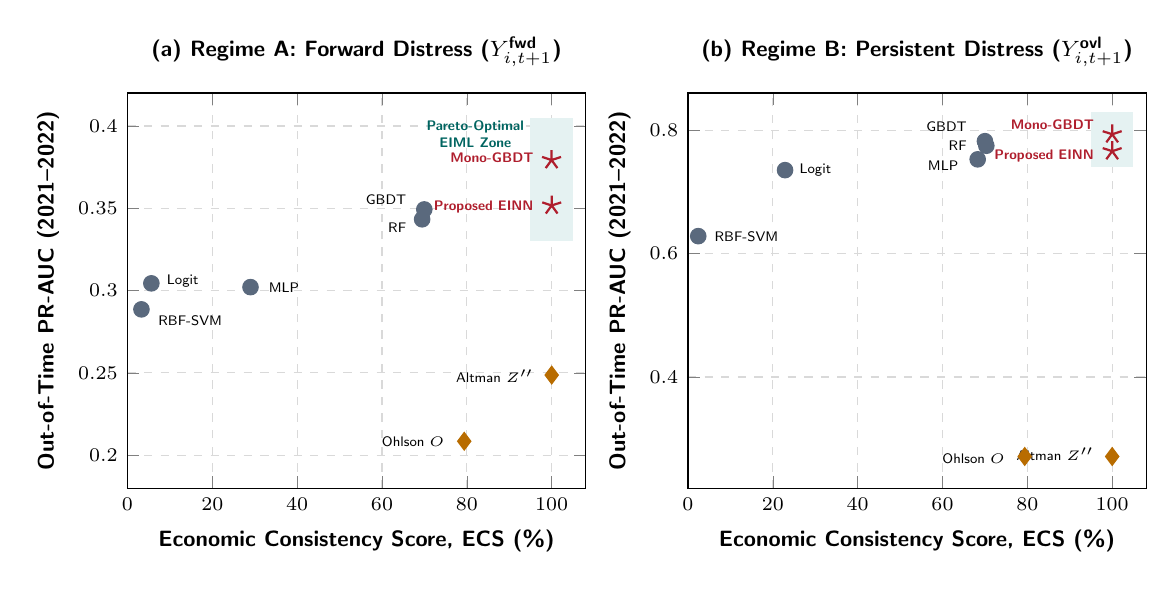
\begin{tikzpicture}
% Left panel: Regime A (Strict Forward Distress Y_fwd)
\begin{axis}[
    name=plotA,
    width=7.4cm,
    height=6.6cm,
    title={\textbf{(a) Regime A: Forward Distress ($Y_{i,t+1}^{\text{fwd}}$)}},
    xlabel={\textbf{Economic Consistency Score, ECS (\%)}},
    ylabel={\textbf{Out-of-Time PR-AUC (2021--2022)}},
    xmin=0, xmax=108,
    ymin=0.18, ymax=0.42,
    grid=both,
    grid style={dashed, gray!30},
    label style={font=\footnotesize\sffamily},
    title style={font=\footnotesize\sffamily},
    ticklabel style={font=\scriptsize}
]
\fill[teal!10] (axis cs:95,0.33) rectangle (axis cs:105,0.405);
\node[font=\tiny\sffamily\bfseries, color=teal!80!black, align=center] at (axis cs:82,0.395) {Pareto-Optimal\\EIML Zone};

% Classical
\addplot[only marks, mark=diamond*, mark size=3.2pt, color=amber!90!black] coordinates {
    (100.0,0.2487)
    (79.38,0.2085)
};
% Unconstrained ML
\addplot[only marks, mark=*, mark size=2.8pt, color=slate] coordinates {
    (5.63,0.3044)
    (3.29,0.2886)
    (69.46,0.3433)
    (69.97,0.3493)
    (29.0,0.3021)
};
% EIML
\addplot[only marks, mark=star, mark options={scale=1.8, thick}, color=crimson] coordinates {
    (99.97,0.3793)
    (100.0,0.3517)
};

\node[font=\tiny\sffamily, anchor=east] at (axis cs:98,0.248) {Altman $Z''$};
\node[font=\tiny\sffamily, anchor=east] at (axis cs:77,0.208) {Ohlson $O$};
\node[font=\tiny\sffamily, anchor=west] at (axis cs:7,0.306) {Logit};
\node[font=\tiny\sffamily, anchor=west] at (axis cs:5,0.282) {RBF-SVM};
\node[font=\tiny\sffamily, anchor=west] at (axis cs:31,0.302) {MLP};
\node[font=\tiny\sffamily, anchor=east] at (axis cs:68,0.338) {RF};
\node[font=\tiny\sffamily, anchor=east] at (axis cs:68,0.355) {GBDT};
\node[font=\tiny\sffamily\bfseries, color=crimson, anchor=east] at (axis cs:98,0.381) {Mono-GBDT};
\node[font=\tiny\sffamily\bfseries, color=crimson, anchor=east] at (axis cs:98,0.351) {Proposed EINN};
\end{axis}

% Right panel: Regime B (Persistent Distress Y_ovl)
\begin{axis}[
    name=plotB,
    at={(plotA.east)}, anchor=west, xshift=1.3cm,
    width=7.4cm,
    height=6.6cm,
    title={\textbf{(b) Regime B: Persistent Distress ($Y_{i,t+1}^{\text{ovl}}$)}},
    xlabel={\textbf{Economic Consistency Score, ECS (\%)}},
    ylabel={\textbf{Out-of-Time PR-AUC (2021--2022)}},
    xmin=0, xmax=108,
    ymin=0.22, ymax=0.86,
    grid=both,
    grid style={dashed, gray!30},
    label style={font=\footnotesize\sffamily},
    title style={font=\footnotesize\sffamily},
    ticklabel style={font=\scriptsize}
]
\fill[teal!10] (axis cs:95,0.74) rectangle (axis cs:105,0.83);

% Classical
\addplot[only marks, mark=diamond*, mark size=3.2pt, color=amber!90!black] coordinates {
    (100.0,0.2713)
    (79.38,0.2713)
};
% Unconstrained ML
\addplot[only marks, mark=*, mark size=2.8pt, color=slate] coordinates {
    (22.88,0.7351)
    (2.42,0.6282)
    (70.33,0.7746)
    (70.0,0.782)
    (68.29,0.7526)
};
% EIML
\addplot[only marks, mark=star, mark options={scale=1.8, thick}, color=crimson] coordinates {
    (100.0,0.7932)
    (100.0,0.7658)
};

\node[font=\tiny\sffamily, anchor=east] at (axis cs:98,0.275) {Altman $Z''$};
\node[font=\tiny\sffamily, anchor=east] at (axis cs:77,0.268) {Ohlson $O$};
\node[font=\tiny\sffamily, anchor=west] at (axis cs:24,0.735) {Logit};
\node[font=\tiny\sffamily, anchor=west] at (axis cs:4,0.628) {RBF-SVM};
\node[font=\tiny\sffamily, anchor=east] at (axis cs:66,0.742) {MLP};
\node[font=\tiny\sffamily, anchor=east] at (axis cs:68,0.774) {RF};
\node[font=\tiny\sffamily, anchor=east] at (axis cs:68,0.805) {GBDT};
\node[font=\tiny\sffamily\bfseries, color=crimson, anchor=east] at (axis cs:98,0.808) {Mono-GBDT};
\node[font=\tiny\sffamily\bfseries, color=crimson, anchor=east] at (axis cs:98,0.758) {Proposed EINN};
\end{axis}
\end{tikzpicture}
\end{document}
